\section{Produktfamilie VisuNet}
\begin{wrapfigure}{r}{0.2\textwidth}
    \vspace{-1.2cm}
    \begin{center}
      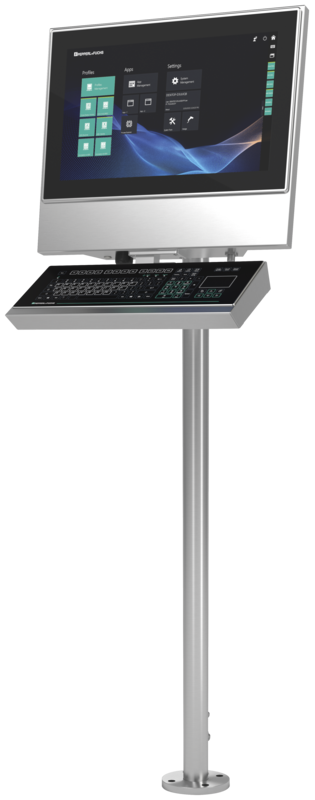
\includegraphics[width=0.2\textwidth]{VisunetFLX.PNG}
    \end{center}
    \vspace{-0.5cm}
    \caption{Pepperl+Fuchs VisuNEt FLX}
    \label{fig:VisuNetFLX}
    \vspace{-0.5cm}
  \end{wrapfigure}
Zielhardware für das Healthmonitoring System sind die \ac{p+f} VisuNet FLX und GXP Platformen. Diese sind Bedien- und Beobachtungssystemen für Explosionsgefährdete bereiche. Din diese Berreichen ist der einsatz von 

\subsection{VisuNet FLX \& GXP}

\subsection{VisuNet RM Shell \& Control Center}